\note{Some things not yet added to thesis skeleton:}
* AEI simulations of auto-alignment of single arm test (appendix?)
* Crystalline coatings in AEI 10m prototype
  * Comparison of GWINC crystalline/amorphous noise to Tara's code, plots of Advanced LIGO mirrors matching Matt Evans' 2008 paper, plots matching Cole paper...
  * AEI mirror crystalline thermal noise plot(s), i.e. the ones I sent Harald in early 2015 - see AEI labbook
  * See email from Ken (2015-06-01 09:27 "Re: Thesis plan uploaded"
* Arduino coil drivers
  * Requirements, how it replaces existing system
  * Board layout
  * First iteration:
    * Performance/screenshots/client-server design
    * Show how it rung up suspension modes when moving by one coarse step
      * Explain physically, i.e. step function is infinitely many sine waves in Fourier domain
  * Second iteration:
    * Show ramp tests where fine steps are taken between coarse steps
    * GUI improvements, like custom groupings of coils
* Speedmeter mirror thermal noise for different layer configurations (i.e. MATLAB scripts that I made already)
* Mirrors with similar reflectivity for different polarisations...?

\chapter{Gravitational Waves}
\label{c:gw-detection}

* Section on DOFs, both for a DRMI and angular DOFs (for benefit of alignment appendix)

\section{Event GW150914}
\checkme{One billion years ago}, a pair of black holes, one with 36 solar masses and another with 29 solar masses, merged into a single black hole with 62 solar masses. The missing energy equivalent to 3 solar masses was radiated away in the form of gravitational waves.

At 09:50:45 \gls{UTC} on \nth{14} September 2015, gravitational waves from the black hole passed through the LIGO Livingston detector, perturbing the mirrors by \checkme{\SI{e-18}{\meter}} and creating a signal large enough for the electronics controlling the interferometer to detect the ripple in space time more than \checkme{23} times above the noise. Seven milliseconds later, the same wavefront passed the LIGO Hanford detector and moved the mirrors in the opposite direction. At that moment, for the first time in human history, a gravitational wave had been detected.

From the gravitational waveform witnessed at the LIGO sites it was possible to determine the type and parameters of the waves' source. \emph{GW150914}'s waveform can be observed in Figure\,\note{ADD FIGURE}. This waveform, consistent with a binary black hole merger, swept up in frequency (the \emph{inspiral}) before combining (the \emph{merger}) and creating an audible ``chirp''. The signal was only above each detector's noise level from a frequency of around \checkme{x}. Not only did LIGO make the first observation of a gravitational wave, it also made the first detection of a binary black hole system. The window into the universe opening up due to the LIGO\textemdash and the worldwide network of gravitational wave detectors in operation and under assembly, GEO-600, Virgo and KAGRA\textemdash represents a new opportunity to study the universe in a completely different way. Some secrets have already been learned, but there are surely many more to be uncovered. Although this is just the beginning of gravitational astronomy, work is already under way to produce bigger and better gravitational wave detectors both on the Earth and in Space.

\section{General Relativity and Gravitational Waves}

One hundred years ago, the landscape in the field of physics was dominated by two physical theories: that of universal gravitation, by Newton, and that of electromagnetism, by Maxwell. Although Newton's theory explained with great precision the motion of objects from apples to planets, it did not reconcile the prediction from Maxwell that the speed of light is constant: a prediction hinted experimentally in the late 19th Century by Michelson and Morley. In 1905, Albert Einstein published his Special Theory of Relativity, implying alongside a wide range of other consequences that space and time are linked in a single continuum known as spacetime. The finite speed of light and the existence of spacetime, however, did not accommodate the idea from Newton that gravity was instantaneous attraction between matter across universal distances, nor did it fix the age-old problem with Newtonian mechanics in explaining the apparent precession of the planet Mercury's orbit. Einstein's later work, his General Theory of Relativity, extended Special Relativity to include strong gravitational attraction, and in doing so he solved the problem with Mercury's orbit and predicted the existence of gravitational waves that dictate how matter should move in spacetime.

\note{Placeholder for text on how GWs are produced}

\subsection{Sources}
Gravitational waves from any Earth-bound object, including the Earth itself, are not even remotely detectable. The strain in spacetime produced by such objects is so weak that there is no hope for us to make such a detection with any known technology. A good estimate for the strain produced by a pair of rotating objects is given in \cite{Sathyaprakash2009} as\footnote{Note that the equation in question, (9) in \cite{Sathyaprakash2009}, has been converted here into SI units.}:
\begin{equation}
  \label{eq:happrox}
  h \lesssim \frac{2 G \left( M v^{2} \right)_{\text{nonspherical}}}{c^4 r},
\end{equation}
where $G$ is the gravitational constant, $\left( M v^{2} \right)_{\text{nonspherical}}$ is the kinetic energy associated with the non-spherical parts of the source, $c$ is the speed of light and $r$ is the distance to the source. To get an idea of what the spacetime strain would be for man-made sources, we can consider as in \cite{Sathyaprakash2009} the case of two cars of mass $M = \SI{e3}{\kilo\gram}$ attached to opposite ends of a rod of length $d = \SI{10}{\meter}$, spinning about its centre in a centrifuge at a frequency of $f = \SI{10}{\hertz}$. The tangential velocity of the cars will be around $2 \pi f d \approx \SI{600}{\meter\per\second}$. Placing the detector one wavelength away, and using Equation\,\ref{eq:happrox}, the strain turns out to be around $\SI{4e-43}{}$. To be able to detect such a strain, Advanced LIGO would require an improvement in sensitivity of \SI{20}{} orders of magnitude, which is clearly ludicrous.

It is only the waves produced by the most massive objects in the universe which we have any chance of detecting: black holes, neutron stars and supernovae, amongst others. Even then, gravitational radiation is only produced by \checkme{the presence of a quadropolar moment} within the source, which means that in general only a subset of sources that happen to be in coalescence or contain surface asymmetries will produce waves.

\subsubsection{Compact Binary Coalescence}
As detected by LIGO in 2016...

\note{Show a picture of the waveform, with annotations - it might be available from https://wiki.ligo.org/viewauth/EPO/DiscoveryTalks.}

\subsubsection{Core Collapse}
\note{Look up numbers from that rates paper.}

\subsubsection{Continuous Wave}
\note{Pulsars}

\subsubsection{Stochastic Background}
CMB...

\note{Make a table of the rules of thumb for strains produced by each source, a la Sathya's article.}

\subsection{Source Localisation}
\note{See Section 2.3 of Sathya's Living Review. Don't go into detail about the type of detector, just the position on Earth.}

\section{Development of the Gravitational Wave Detector}
The field of experimental gravitational wave detection began with Joseph Weber's studies in the 1960s \cite{Weber1960}. His \emph{Weber bar} was developed to act as a strain meter, with piezoelectric sensors placed on the surface of an aluminium cylinder to convert changes in length into electrical signals. Whilst the expected change in length of such a cylinder from gravitational radiation would in most cases be tiny---\checkme{of the order \SI{1e-22}{\meter} for a particularly loud source}---the resonant frequency of the cylinder, typically in the kilohertz range, acts to enhance the amplitude of the length change. The sensitivity of such a bar as a function of frequency is determined in part by its quality factor (Q), with a necessary trade-off being made between peak sensitivity (high Q) and detection bandwidth (low Q). As sources of gravitational radiation are almost universally weak, the only reasonable hope of making such a detection is to choose a high Q material and hope for a favourable signal frequency.

\begin{wrapfigure}{r}{0.5\textwidth}
  \includegraphics[width=0.5\textwidth]{10-introduction/graphics/dynamic/michelson.pdf}
  \caption{Blah blah blah}
\end{wrapfigure}

The original resonant bar detectors were evolved over time to become cryogenic, to decrease the effect of thermal noise; and spherical, to maximise the test mass's Q. Despite such improvements the peak sensitivity of state-of-the-art resonant bar detectors was surpassed by interferometric gravitational wave detectors in 2003 \cite{Pitkin2011} after it was shown that second generation detectors would offer superior sensitivity across a much wider bandwidth\footnote{Interestingly, a Weber bar had a particularly high profile opportunity to make the first detection. One was contained in the scientific payload of Apollo 17 with the intention to observe gravitational radiation from the low seismic noise environment of the Moon. Unfortunately a manufacturing error led to a failure in the experiment.} \cite{Harry2002a}. The interferometer was first suggested as a means for gravitational wave detection shortly after the introduction of the Weber bar\footnote{The first known example being by Gertsenshtein and Pustovoit in the Soviet \emph{Journal of Experimental and Theoretical Physics} in 1962.}, but efforts to build prototypes and understand the significant sources of noise only gained momentum in the 1970s (see for example Moss \etal \cite{Moss1971} from 1971 or Weiss \cite{Weiss1972} from 1972).

% Search 'Lunar Surface Gravimeter' for Moon bar detector details

\subsection{The Gravitational Wave Interferometer}
%* First interferometric detectors:
%  * Drever, Hough, Glasgow and Munich stuff
%  * Glasgow 10m, Caltech 40m, Garching 30m, etc.
%  * Formation of LIGO and GEO collaborations
%  * Foundational papers (Weiss noise analysis, conference presentations from Schilling and Drever, etc.)
%  * Meers paper on signal recycling
%  * Initial LIGO, GEO-600, TAMA, Virgo, etc.
%  * Enhanced LIGO (and Enhanced Virgo?)

Over the course of the 1980s the \MI (see Figure\,\ref{fig:mi}) was developed into a very respectable gravitational wave detection apparatus.

\begin{figure}
  \begin{center}
    \begin{subfigure}{.3\textwidth}
      \includegraphics[width=\columnwidth]{10-introduction/graphics/dynamic/michelson.pdf}
      \caption{Simple \MI}
      \label{fig:mi}
    \end{subfigure}
    \hfill
    \begin{subfigure}{.3\textwidth}
      \includegraphics[width=\columnwidth]{10-introduction/graphics/dynamic/fabry-perot-michelson.pdf}
      \caption{\FPMI}
      \label{fig:fpmi}
    \end{subfigure}
    \hfill
    \begin{subfigure}{.3\textwidth}
      \includegraphics[width=\columnwidth]{10-introduction/graphics/dynamic/dual-recycled-fabry-perot-michelson.pdf}
      \caption{\DRFPMI}
      \label{fig:drfpmi}
    \end{subfigure}
    \caption[The evolution of the gravitational wave detector]{The evolution of the gravitational wave detector. Figure\,\ref{fig:mi} shows the simple \MI used since the famous Michelson and Morley experiments of the 1880s, and proposed for gravitational wave detection in early literature. Figure\,\ref{fig:fpmi} shows a \MI with the addition of \FP arm cavities to enhance sensitivity. Figure\,\ref{fig:drfpmi} shows a \FPMI with the addition of recycling mirrors.}
  \end{center}
\end{figure}

\subsection{Pulsar Timing}
\note{Short note on pulsar timing arrays.}

\section{Thesis Structure}

This thesis will be structured as follows...

\begin{figure}
  \includegraphics[width=\columnwidth]{10-introduction/graphics/dynamic/thesis-structure.pdf}
  \caption{Thesis structure}
  \label{fig:thesis-structure}
\end{figure}